% ============================================================
%  SCHOLA DOMESTICA — Magister Mathematica
%  Level 1 | Week 8 | Day 4
%  Topic: Addition and Subtraction Together
%  (Opposites; first glimpse of inverse relationship;
%   +/− mixed facts to 10)
% ============================================================
\documentclass[12pt, letterpaper]{article}

\usepackage[top=1in, bottom=1in, left=1in, right=1in]{geometry}
\usepackage{fontenc}
\usepackage{inputenc}
\usepackage{lmodern}
\usepackage{microtype}
\usepackage{amsmath}
\usepackage{graphicx}
\usepackage{xcolor}
\usepackage{tikz}
\usepackage{array}
\usepackage{enumitem}
\usepackage{multicol}
\usepackage{mdframed}
\usepackage{fancyhdr}

\definecolor{scholared}{RGB}{160,30,30}
\definecolor{scholagold}{RGB}{180,140,40}
\definecolor{scholacream}{RGB}{253,248,235}
\definecolor{scholagreen}{RGB}{50,110,60}
\definecolor{scholablue}{RGB}{40,80,140}

\pagestyle{fancy}
\fancyhf{}
\renewcommand{\headrulewidth}{0.6pt}
\fancyhead[L]{\small\textcolor{scholared}{\textbf{Schola Domestica — Magister Mathematica}}}
\fancyhead[R]{\small\textcolor{scholared}{Level 1 · Week 8 · Day 4}}
\fancyfoot[C]{\small\textcolor{gray}{— \thepage\ —}}

\newcommand{\answerline}{\underline{\hspace{2.5cm}}}
\newcommand{\biganswerline}{\underline{\hspace{4cm}}}
\newcommand{\numbox}{\fbox{\hspace{0.6cm}\vphantom{0}}}

\newmdenv[
  backgroundcolor=scholacream,
  linecolor=scholared,
  linewidth=1.5pt,
  roundcorner=6pt,
  innertopmargin=8pt,
  innerbottommargin=8pt,
  innerleftmargin=10pt,
  innerrightmargin=10pt
]{lessonbox}

\begin{document}

\begin{center}
  {\LARGE\textbf{\textcolor{scholared}{Addition and Subtraction Together}}}\\[4pt]
  {\Large\textcolor{scholagold}{\textit{Opposites — Forward and Back}}}\\[6pt]
  {\small Name: \biganswerline \hspace{1cm} Date: \answerline}
\end{center}

\vspace{4pt}
\noindent\textcolor{scholared}{\rule{\linewidth}{1pt}}
\vspace{4pt}

% IMAGE PROMPT (Miyazaki-style watercolour):
% A wooden seesaw in a sunny garden. On the left side sits a group of 4 red apples; on the
% right side sits a group of 3 green apples. The seesaw is tilted. Two children watch.
% Soft bright watercolour, morning light. No numerals.

\begin{lessonbox}
\textbf{Addition and Subtraction are opposites.}\\[4pt]
Addition goes \textbf{forward} on the number line. Subtraction goes \textbf{backward}.\\[6pt]
\begin{center}
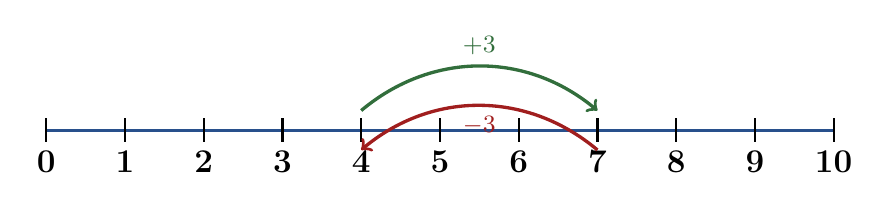
\begin{tikzpicture}[scale=1.0]
  \draw[very thick, scholablue] (0,0) -- (10,0);
  \foreach \n in {0,...,10} {
    \draw[thick] (\n,0.15) -- (\n,-0.15);
    \node[below=4pt] at (\n,0) {\large\textbf{\n}};
  }
  % +3 forward from 4
  \draw[->, very thick, scholagreen, bend left=40] (4,0.25) to node[above]{\small $+3$} (7,0.25);
  % -3 backward from 7
  \draw[->, very thick, scholared, bend right=40] (7,-0.25) to node[below]{\small $-3$} (4,-0.25);
\end{tikzpicture}
\end{center}
\medskip
$4 + 3 = 7$ \hspace{1cm} $7 - 3 = 4$ \hspace{1cm} \textit{They undo each other!}
\end{lessonbox}

\bigskip

% ===== PART I: PAIRS =====
\noindent\textcolor{scholared}{\large\textbf{Part I — Addition and Subtraction Pairs}} \hfill \textit{(Problems 1–4)}

\medskip\noindent\textit{Complete both sentences using the same three numbers.}

\bigskip
\noindent\textbf{1.} \quad $3 + 5 = $ \numbox \hspace{2cm} $8 - 5 = $ \numbox

\bigskip
\noindent\textbf{2.} \quad $6 + 2 = $ \numbox \hspace{2cm} $8 - 2 = $ \numbox

\bigskip
\noindent\textbf{3.} \quad $4 + 4 = $ \numbox \hspace{2cm} $8 - 4 = $ \numbox

\bigskip
\noindent\textbf{4.} \quad $7 + 3 = $ \numbox \hspace{2cm} $10 - 3 = $ \numbox

\bigskip
\noindent\textcolor{scholared}{\rule{\linewidth}{0.4pt}}

% ===== PART II: MIXED FACTS =====
\noindent\textcolor{scholared}{\large\textbf{Part II — Mixed + and − Facts}} \hfill \textit{(Problems 5–14)}

\bigskip
\begin{multicols}{2}
\noindent\textbf{5.} $\; 6 + 3 = $ \numbox \\[10pt]
\noindent\textbf{6.} $\; 9 - 4 = $ \numbox \\[10pt]
\noindent\textbf{7.} $\; 5 + 4 = $ \numbox \\[10pt]
\noindent\textbf{8.} $\; 7 - 3 = $ \numbox \\[10pt]
\noindent\textbf{9.} $\; 2 + 6 = $ \numbox

\columnbreak

\noindent\textbf{10.} $\; 8 - 6 = $ \numbox \\[10pt]
\noindent\textbf{11.} $\; 4 + 5 = $ \numbox \\[10pt]
\noindent\textbf{12.} $\; 10 - 5 = $ \numbox \\[10pt]
\noindent\textbf{13.} $\; 3 + 7 = $ \numbox \\[10pt]
\noindent\textbf{14.} $\; 6 - 6 = $ \numbox
\end{multicols}

\bigskip
\noindent\textcolor{scholared}{\rule{\linewidth}{0.4pt}}

% ===== PART III: WORD PROBLEMS =====
\noindent\textcolor{scholared}{\large\textbf{Part III — Word Problems}} \hfill \textit{(Problems 15–16)}

\bigskip
\noindent\textbf{15.} Clara bakes 5 biscuits and then bakes 4 more. She eats 2. How many are left?

\medskip
\hspace{2em} First: $5 + 4 = $ \numbox \hspace{1cm} Then: \numbox $ - 2 = $ \numbox

\bigskip
\noindent\textbf{16.} There are 10 birds on a wire. 3 fly away, then 2 more arrive.\\
How many birds are on the wire now?

\medskip
\hspace{2em} $10 - 3 = $ \numbox \hspace{1cm} \numbox $+ 2 = $ \numbox

\end{document}
